\documentclass{article}

\usepackage[francais]{babel}
\usepackage[T1]{fontenc}
\usepackage[latin1]{inputenc}
\usepackage[left=1cm, right=1cm, top=6mm, bottom=6mm]{geometry}
\usepackage{float}
\usepackage{graphicx}
\usepackage{array}
\usepackage{multirow}
\usepackage{amsmath, amssymb, mathrsfs}

\begin{document}

\begin{flushleft}
NOM PRENOM: \ldots \ldots \ldots \ldots \ldots \ldots \ldots \ldots \ldots

\bigskip
\end{flushleft}
\begin{center}
{\fbox{$2^{de}5$ \qquad \qquad \textbf{\Large{Contr�le de cours 6 (sujet 1)}}
\qquad \qquad 07/05/2009}}
\end{center}


\bigskip

\begin{enumerate}
  \item Tracer la courbe repr�sentative de la fonction carr� sur $\mathbb{R}$.
  
  \begin{center}
  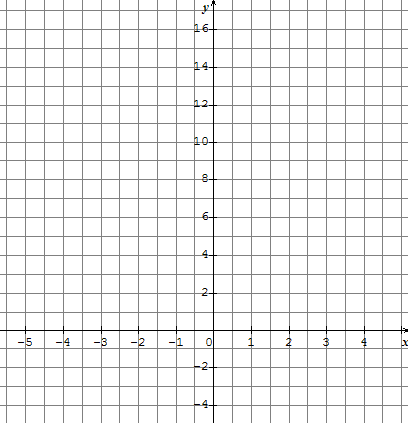
\includegraphics[width=9cm]{images/ex1.png}
  \end{center}

  Comment s'appelle ce type de courbe? 
  
  \bigskip
  
  \bigskip
  
  \item Donner le domaine de d�finition $D$ de la fonction inverse puis son
  tableau de variation sur $D$.
  
  \bigskip
  
  \bigskip
  
  \bigskip
  
  
  \bigskip
  
  \bigskip
  
  
  \bigskip
  
  \item Donner la d�finition de fonction d�croissante sur un intervalle $I$.
  
  \bigskip
  
  \bigskip
  
  
  \bigskip
  
  \bigskip
  
  
  \item La courbe repr�sentative de la fonction inverse a une sym�trie. De
  quelle sym�trie s'agit-il? Quel nom donne t-on aux fonctions ayant cette particularit�
  graphique?
  
  \bigskip
  
  \bigskip
  
  \bigskip
  
  \bigskip
  
  
  \item R�soudre $(x-1)^2=9$.
\end{enumerate}


\pagebreak

\begin{flushleft}
NOM PRENOM: \ldots \ldots \ldots \ldots \ldots \ldots \ldots \ldots \ldots

\bigskip
\end{flushleft}
\begin{center}
{\fbox{$2^{de}5$ \qquad \qquad \textbf{\Large{Contr�le de cours 6 (sujet 2)}}
\qquad \qquad 07/05/2009}}
\end{center}


\bigskip

\begin{enumerate}
  \item Donner le domaine de d�finition $D$ de la fonction inverse.
  
  \bigskip
  
  Tracer la courbe repr�sentative de la fonction inverse sur $D$.
  
  \begin{center}
  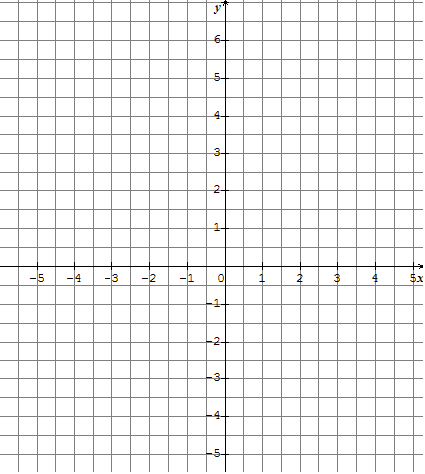
\includegraphics[width=9cm]{images/ex2.png}
  \end{center}

  Comment s'appelle ce type de courbe? 
  
  \bigskip
  
  \bigskip
  
  \item Donner le tableau de variation de la fonction carr� sur $\mathbb{R}$.
  
  \bigskip
  
  \bigskip
  
  \bigskip
  
  
  \bigskip
  
  \bigskip
  
  
  \bigskip
  
  \item Donner la d�finition de fonction croissante sur un intervalle $I$.
  
  \bigskip
  
  \bigskip
  
  
  \bigskip
  
  \bigskip
  
  
  \item La courbe repr�sentative de la fonction carr� a une sym�trie. De
  quelle sym�trie s'agit-il? Quel nom donne t-on aux fonctions ayant cette particularit�
  graphique?
  
  \bigskip
  
  \bigskip
  
  \bigskip
  
  \bigskip
  
  
  \item R�soudre $(x-2)^2=16$.
\end{enumerate}

\end{document}
